\documentclass[border=7pt]{standalone}
\usepackage{amsmath,amssymb,bm,mathtools}
\usepackage[fontset=none]{ctex}
\setCJKmainfont{Songti SC}\setCJKsansfont{PingFang SC}
\usepackage{tikz}\usetikzlibrary{arrows.meta,calc,patterns,angles,quotes,decorations.markings,decorations.pathmorphing}
\newcommand{\dd}{\mathop{}\!\mathrm d}
\definecolor{blue}{HTML}{235789}\definecolor{red}{HTML}{BC4B41}
\tikzset{axis/.style={->,>=Stealth,line width=.55pt},world/.style={line width=.9pt},flow/.style={->,>=Stealth,line width=.85pt},ray/.style={->,>=Stealth,line width=.85pt},guide/.style={dashed,line width=.4pt},aux/.style={dashed,line width=.4pt},dim/.style={<->,>=Stealth,line width=.5pt},every node/.style={font=\normalsize},force/.style={->,>=Stealth,very thick},gas/.style={fill=blue!7}}
\begin{document}
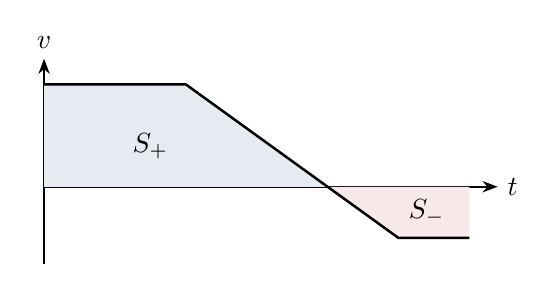
\begin{tikzpicture}[x=.9cm,y=.65cm]
\draw[axis](0,0)--(6.4,0)node[right]{$t$};\draw[axis](0,-1.5)--(0,2.5)node[above]{$v$};
\fill[blue!12](0,0)--(0,2)--(2,2)--(4,0)--cycle;\fill[red!12](4,0)--(5,-1)--(6,-1)--(6,0)--cycle;
\draw[world](0,2)--(2,2)--(5,-1)--(6,-1);\node at(1.5,.8){$S_+$};\node at(5.4,-.5){$S_-$};\end{tikzpicture}
\end{document}
